\documentclass{beamer}
\usetheme{metropolis}
\usepackage{graphicx}
\usepackage{subfig}
\usepackage{tcolorbox}
\title{Calculus-Based Physics-2: Electricity, Magnetism, and Thermodynamics (PHYS180-02): Unit 5}
\author{Jordan Hanson}
\institute{Whittier College Department of Physics and Astronomy}

\begin{document}
\maketitle

\section{Unit 4 Review}

\begin{frame}{Unit 4 Summary}
\textbf{Reading: Chapters 7, 9, and 10}
\begin{enumerate}
\item \alert{Voltage and Capacitance}
\item Ohm's Law
\item DC circuits
\end{enumerate}
\end{frame}

\section{Unit 4 Review Problems}

\begin{frame}{Unit 4 Review Problems}
\begin{columns}[T]
\begin{column}{0.5\textwidth}
Which of the following would decrease the time required to charge the capacitor at right?
\begin{itemize}
\item A: Decreasing the capacitance
\item B: Decreasing the resistance
\item C: It already charges as fast as possible
\item D: Both A and B
\end{itemize}
\end{column}
\begin{column}{0.5\textwidth}
\begin{figure}
\centering
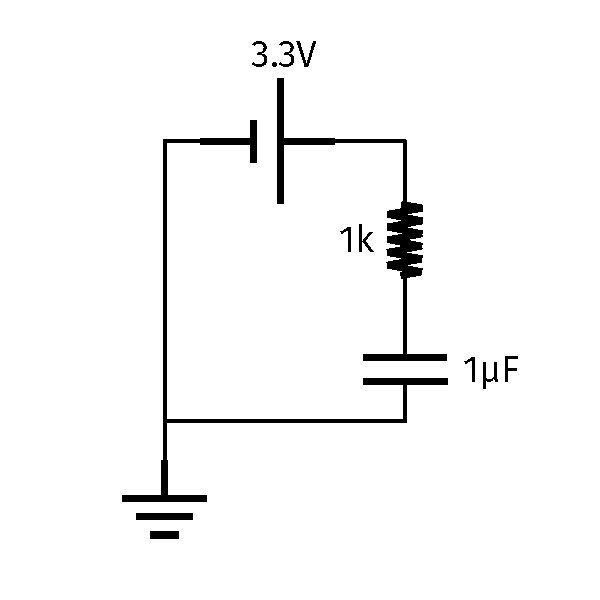
\includegraphics[width=0.8\textwidth]{figures/iVCurve7.pdf}
\caption{\label{fig:RC0} An RC circuit.}
\end{figure}
\end{column}
\end{columns}
\end{frame}

\begin{frame}{Unit 4 Review Problems}
\begin{columns}[T]
\begin{column}{0.5\textwidth}
What is the RC time of the circuit?
\begin{itemize}
\item A: 1 $\mu$s
\item B: 1 ms
\item C: 1 s
\item D: 10 s
\end{itemize}
\end{column}
\begin{column}{0.5\textwidth}
\begin{figure}
\centering
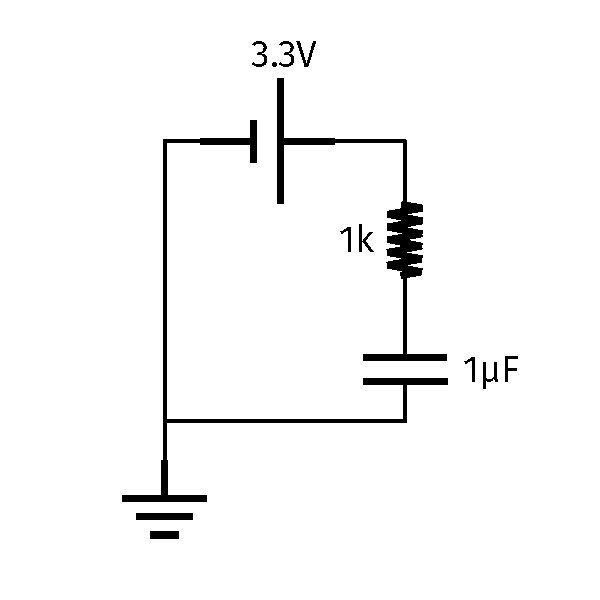
\includegraphics[width=0.8\textwidth]{figures/iVCurve7.pdf}
\caption{\label{fig:RC1} An RC circuit.}
\end{figure}
\end{column}
\end{columns}
\end{frame}

\begin{frame}{Unit 4 Review Problems}
\begin{columns}[T]
\begin{column}{0.5\textwidth}
What is the maximum charge stored eventually in the capacitor?  \textit{Recall that $Q = CV$}.
\begin{itemize}
\item A: 3.3 $\mu$ C
\item B: 1.5 $\mu$ C
\item C: 3.3 mC
\item D: 1.5 C
\end{itemize}
\end{column}
\begin{column}{0.5\textwidth}
\begin{figure}
\centering
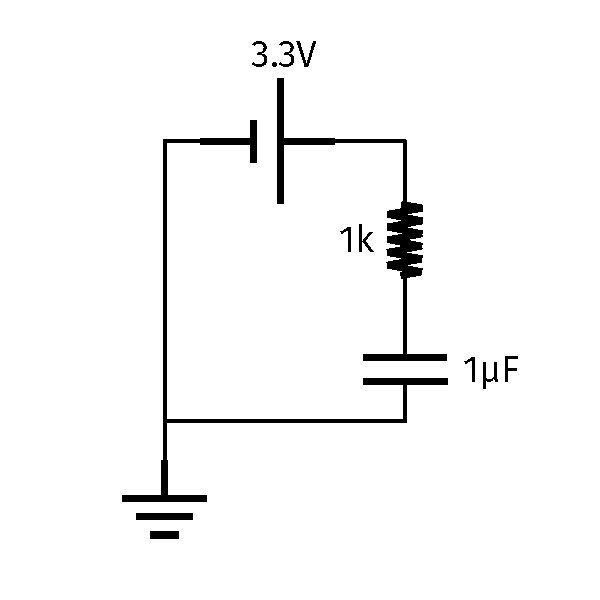
\includegraphics[width=0.8\textwidth]{figures/iVCurve7.pdf}
\caption{\label{fig:RC2} An RC circuit.}
\end{figure}
\end{column}
\end{columns}
\end{frame}

\section{Summary}

\begin{frame}{Unit 5 Summary}
\textbf{Reading: Chapter 11}
\begin{enumerate}
\item Magnetism and magnetic fields
\item \alert{Motion of a charged particle in a magnetic field}
\item Other forces
\item Current loops
\end{enumerate}
\end{frame}

\section{Magnetism and magnetic fields}

\begin{frame}{Magnetism and magnetic fields}
\begin{figure}
\centering
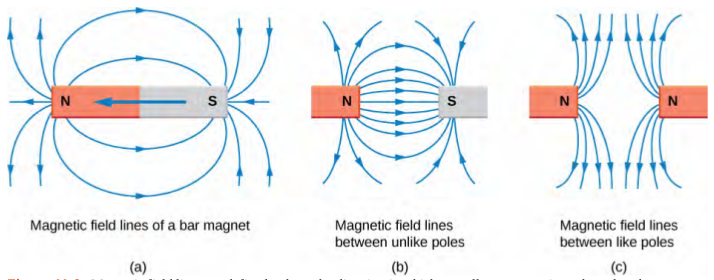
\includegraphics[width=0.9\textwidth,trim=0cm 1cm 0cm 0cm,clip=true]{figures/fields1.png}
\caption{\label{fields1} Various magnetic field line configurations.}
\end{figure}
\end{frame}

\begin{frame}{Magnetism and magnetic fields}
\begin{figure}
\centering
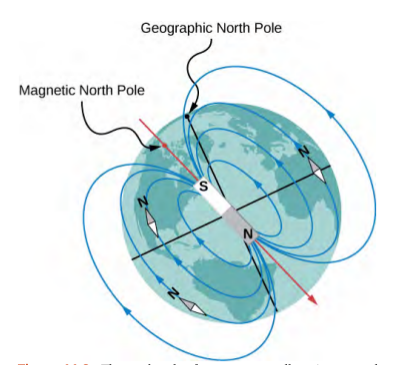
\includegraphics[width=0.6\textwidth,trim=0cm 0.1cm 0cm 0cm,clip=true]{figures/fields2.png}
\caption{\label{fields2} The magnetic and geographic poles are not the same.}
\end{figure}
\end{frame}

\begin{frame}{Magnetism and magnetic fields}
It would be nice if we could say:
\begin{equation}
F = \mu_0 \frac{q_{m,1} g_{m,2}}{r^2}
\end{equation}
But...we can't.  Why?  There's no such thing has magnetic charge:
\begin{align}
\nabla \cdot \vec{E} &= \rho/\epsilon_0 \\ 
\nabla \cdot \vec{B} &= 0
\end{align}
But there is a force associating charge and magnetic fields.  But first, let's review the cross-product.
\end{frame}

\begin{frame}{Magnetism and magnetic fields}
What is a cross-product and how does it work? \\ \vspace{0.25cm}
\begin{figure}
\centering
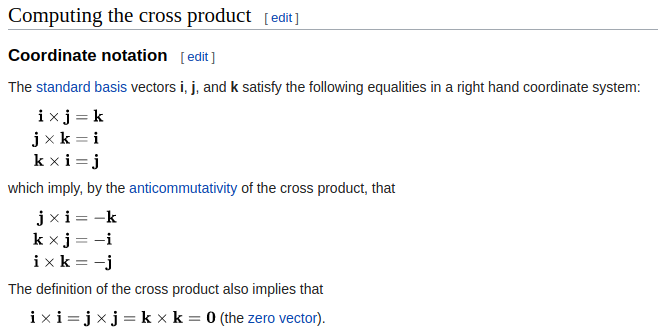
\includegraphics[width=0.75\textwidth]{figures/crossP.png}
\caption{\label{fig:crossP} The cross-product is a way of multiplying unit vectors.}
\end{figure}
\end{frame}

\begin{frame}{Magnetism and magnetic fields}
Let $\vec{v} = 2\hat{i}$ and $w = -2 \hat{j}$.  What is $\vec{v} \times \vec{w}$?
\begin{itemize}
\item A: $-4 \hat{k}$
\item B: $4 \hat{k}$
\item C: $-2 \hat{i}$
\item D: $2 \hat{j}$
\end{itemize}
\end{frame}

\begin{frame}{Magnetism and magnetic fields}
Let $\vec{v} = 3\hat{j}$ and $w = 5 \hat{k}$.  What is $\vec{v} \times \vec{w}$?
\begin{itemize}
\item A: $15 \hat{i}$
\item B: $5 \hat{j}$
\item C: $3 \hat{i}$
\item D: $15 \hat{k}$
\end{itemize}
\end{frame}

\begin{frame}{Magnetism and magnetic fields}
Let $\vec{v} = 3\hat{i} \times 3\hat{j}$ and $w = 2 \hat{k}$.  What is $\vec{v} \times \vec{w}$?
\begin{itemize}
\item A: $-6 \hat{j} + 6\hat{k}$
\item B: $-6 \hat{j} + 6\hat{i}$
\item C: $6 \hat{j} + 6\hat{i}$
\item D: $6 \hat{k} + 6\hat{i}$
\end{itemize}
\end{frame}

\begin{frame}{Magnets and magnetic fields}
\textbf{Group board exercise:} Compute the following cross product:
\begin{align}
\vec{v} &= 2\hat{i}-2\hat{j} \\
\vec{w} &= 4\hat{j}-4\hat{i} \\
\vec{v} \times \vec{w} &= ??
\end{align}
\end{frame}

\begin{frame}{Magnets and magnetic fields}
\textbf{Group board exercise:} Compute the following cross product:
\begin{align}
\vec{v} &= 2\hat{i}-2\hat{j}+\hat{k} \\
\vec{w} &= 4\hat{j}-4\hat{i}-\hat{k} \\
\vec{v} \times \vec{w} &= ??
\end{align}
\end{frame}

\begin{frame}{Magnets and magnetic fields}
\begin{tcolorbox}[colback=white,colframe=red!40!blue,title=The Lorentz Force]
\alert{Let a particle with charge q and velocity $\vec{v}$ move through a magnetic field $\vec{B}$. The Lorentz force on the charged particle is
\begin{equation}
\vec{F}_{\rm L} = q\vec{v} \times \vec{B}
\label{eq:Lorentz}
\end{equation}}
\end{tcolorbox}
\textit{As a helpful memory tool, we have the right-hand rule to
remember the direction of the cross-product.} The units of the
magnetic field are the Telsa, after Nikola Tesla. We also have
the Gauss which is $10^{-4}$ Tesla.
\end{frame}

\begin{frame}{Magnets and magnetic fields}
\begin{figure}
\centering
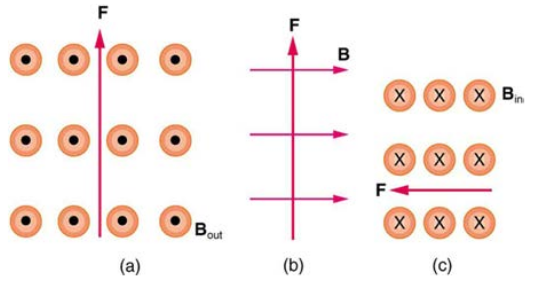
\includegraphics[width=0.75\textwidth]{figures/lorentzProblem.png}
\caption{\label{fig:lorentzProblem} Three different magnetic field and charge scenarios. The
vector $\vec{F}$ is the direction of the Lorentz force, and the magnetic field
is uniform. A dot indicates that the magnetic field is coming out of
the page, and an x indicates that the field is going into the page.}
\end{figure}
\end{frame}

\begin{frame}{Magnets and magnetic fields}
\begin{columns}[T]
\begin{column}{0.3\textwidth}
In which of the diagrams is a positively charged particle moving to the left?
\begin{itemize}
\item A: A
\item B: B
\item C: C
\item D: WAT WAT WAT
\end{itemize}
\end{column}
\begin{column}{0.7\textwidth}
\begin{figure}
\centering
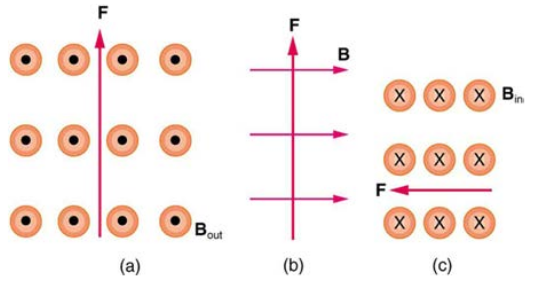
\includegraphics[width=0.75\textwidth]{figures/lorentzProblem.png}
\caption{\label{fig:lorentzProblem2} Three different magnetic field and charge scenarios.}
\end{figure}
\end{column}
\end{columns}
\end{frame}

\begin{frame}{Magnets and magnetic fields}
\begin{columns}[T]
\begin{column}{0.3\textwidth}
In which of the diagrams is a positively charged particle moving upwards?
\begin{itemize}
\item A: A
\item B: B
\item C: C
\item D: WAT WAT WAT
\end{itemize}
\end{column}
\begin{column}{0.7\textwidth}
\begin{figure}
\centering
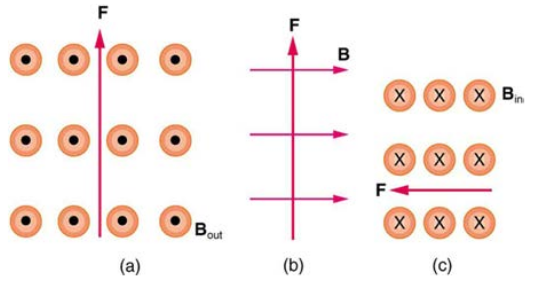
\includegraphics[width=0.75\textwidth]{figures/lorentzProblem.png}
\caption{\label{fig:lorentzProblem3} Three different magnetic field and charge scenarios.}
\end{figure}
\end{column}
\end{columns}
\end{frame}

\begin{frame}{Magnets and magnetic fields}
\begin{columns}[T]
\begin{column}{0.3\textwidth}
In which of the diagrams is a negatively charged particle into the page?
\begin{itemize}
\item A: A
\item B: B
\item C: C
\item D: WAT WAT WAT
\end{itemize}
\end{column}
\begin{column}{0.7\textwidth}
\begin{figure}
\centering
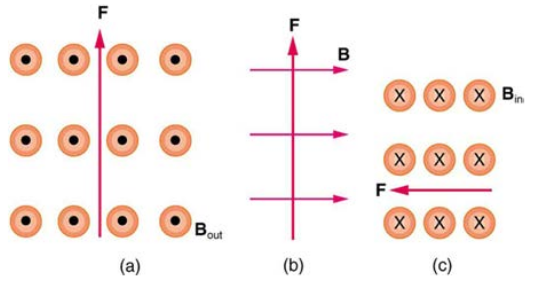
\includegraphics[width=0.75\textwidth]{figures/lorentzProblem.png}
\caption{\label{fig:lorentzProblem4} Three different magnetic field and charge scenarios.}
\end{figure}
\end{column}
\end{columns}
\end{frame}

\begin{frame}{Magnets and magnetic fields}
\begin{columns}[T]
\begin{column}{0.3\textwidth}
In which of the diagrams is a negatively charged particle to the right?
\begin{itemize}
\item A: A
\item B: B
\item C: C
\item D: WAT WAT WAT
\end{itemize}
\end{column}
\begin{column}{0.7\textwidth}
\begin{figure}
\centering
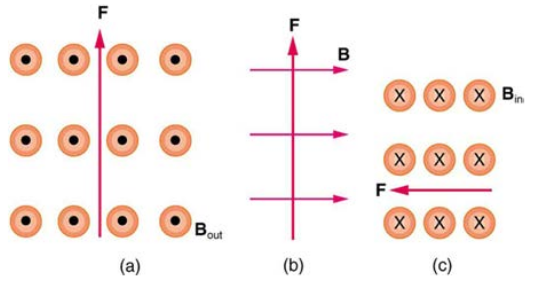
\includegraphics[width=0.75\textwidth]{figures/lorentzProblem.png}
\caption{\label{fig:lorentzProblem5} Three different magnetic field and charge scenarios.}
\end{figure}
\end{column}
\end{columns}
\end{frame}

\begin{frame}{Magnets and magnetic fields}
A theorem for the magnitude of the cross-product:  Let $\vec{a}$ and $\vec{b}$ be vectors and $\theta$ be the angle between them.  The magnitude of the cross product is:
\begin{equation}
|\vec{a} \times \vec{b}| =  a b \sin\theta
\end{equation}
Thus, the magnitude of the Lorentz force is
\begin{equation}
F_{\rm L} = q v B \sin\theta
\end{equation}
The angle $\theta$ is between the velocity and the magnetic field.
\end{frame}

\begin{frame}{Magnets and magnetic fields}
A cosmic ray proton moving toward the Earth at $3 \times 10^{6}$ m/s experiences a magnetic force of $2 \times 10^{-17}$ N. What is the strength of the magnetic field of the Earth? (1 Gauss = $10^{-4}$ Tesla).
\begin{itemize}
\item A: 0.1 Gauss
\item B: 0.6 Gauss
\item C: 1 Gauss
\item D: 6 Gauss
\end{itemize}
\end{frame}

\begin{frame}{Magnets and magnetic fields}
\begin{figure}
\centering
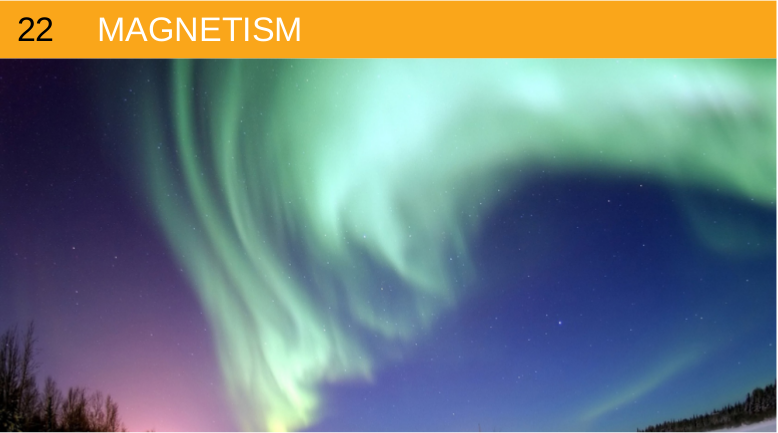
\includegraphics[width=0.9\textwidth]{figures/aurora.png}
\caption{\label{fig:aurora} The aurora borealis, or northern lights.}
\end{figure}
\end{frame}

\begin{frame}{Magnets and magnetic fields}
\begin{figure}
\centering
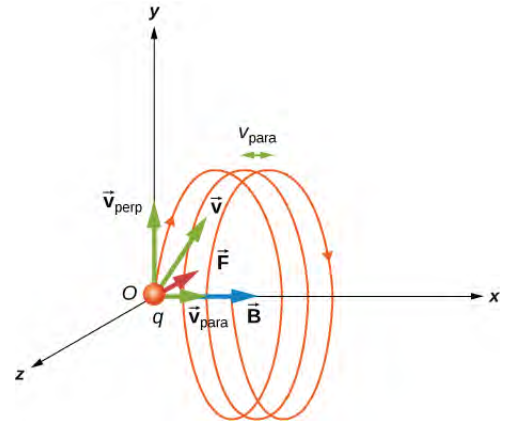
\includegraphics[width=0.5\textwidth]{figures/helix.png}
\caption{\label{fig:helix} In three dimensions, charged particle motion in a $\vec{B}$-field can result in \textit{helical motion}.}
\end{figure}
\end{frame}

\begin{frame}{Magnets and magnetic fields}
Suppose the velocity of a charged particle with mass $m$ is $\vec{v} = v_x \hat{i} + v_z \hat{k}$ through a uniform field $\vec{B} = B\hat{k}$.  The Lorentz force causes centripetal motion and the particle continues to have constant velocity in the $\hat{k}$ direction:
\begin{align}
\vec{F} &= q \vec{v} \times \vec{B} \\
\vec{F} &= -q B v_x \hat{j} \\
m r \omega^2 &= q B v_x \\
\omega &= \sqrt{\frac{qBv_x}{m r}} \\
f &= \frac{1}{2\pi}\sqrt{\frac{qBv_x}{m r}}, ~~ T = 2\pi \sqrt{\frac{m r}{q B v_x}} \\
\vec{v} \cdot \hat{k} &= v_z
\end{align}
\end{frame}

\begin{frame}{Magnets and magnetic fields}
Which of the following is true of a charged particle moving in a helical fashion through a magnetic field?
\begin{itemize}
\item A: Raising the strength of the B-field increases the period
\item B: Raising the strength of the B-field increases the frequency
\item C: The particle has a constant velocity parallel to the field
\item D: B and C
\end{itemize}
\end{frame}

\begin{frame}{Magnets and magnetic fields}
Two particles are moving in helixes through a region where there is a magnetic field.  One moves clockwise as you observe it, and the other moves counter-clockwise, and the helices have about the same radius.  Which of the following is true?
\begin{itemize}
\item A: The particles have identical charge.
\item B: The particles have identical charge, and about the same mass.
\item C: The particles have opposite charge, and about the same mass.
\item D: The particles have different masses.
\end{itemize}
\end{frame}

\begin{frame}{Magnets and magnetic fields}
Same situation: if the B-field strength increases, and the frequency of the rotations stays constant, what happens to the radius of the helices?
\begin{itemize}
\item A: They increase
\item B: They decrease
\item C: The particles have opposite charge, and about the same mass.
\item D: The particles have different masses.
\end{itemize}
\end{frame}

\begin{frame}{Magnets and magnetic fields}
\small
\textbf{Group board exercise:} Recall that the \textit{rotational kinetic energy} of a particle with mass $m$ moving circularly with radius $r$ is
\begin{equation}
K_{rot} = \frac{1}{2}I\omega^2 = \frac{1}{2}mr^2\omega^2
\end{equation}
Show that the \alert{total energy}, including translational and rotational, of the particle moving in the magnetic helix is
\begin{equation}
E_{tot} = \frac{1}{2}m v_z^2 + \frac{1}{2} q v_x r B
\end{equation}
What is the total energy of a proton (mass of $1.6 \times 10^{-27}$ kg), moving with $v_z = 0.1\times 10^{8}$ m/s, $v_x = 1.0 \times 10^{8}$ m/s, and $r = 0.625$ m in a field with $B = 10^{-4}$ Tesla?  What can we say about the field strength if we observe $r$ decreasing and $v_x$ to be constant?
\end{frame}

\begin{frame}{Magnets and magnetic fields}
\begin{figure}
\centering
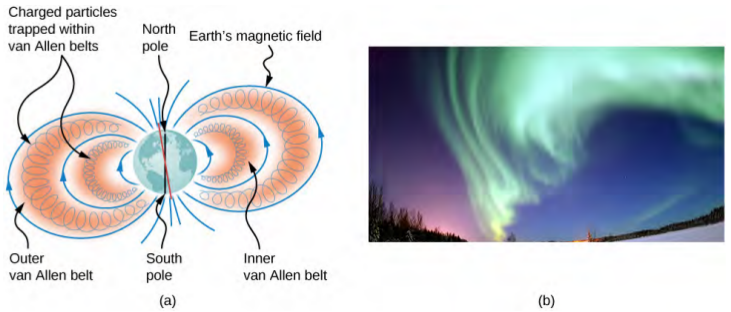
\includegraphics[width=0.85\textwidth]{figures/borealis.png}
\caption{\label{fig:borealis} We observe this effect in the auroras, and the van Allen belts.}
\end{figure}
\end{frame}

\begin{frame}{Magnets and magnetic fields}
A cool talk on the aurora borealis:
\url{https://youtu.be/czMh3BnHFHQ} \\
\begin{figure}
\centering
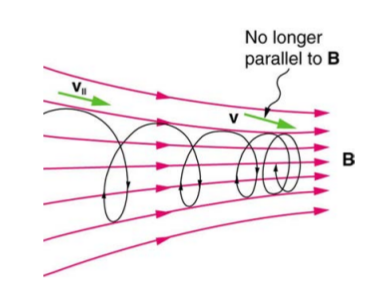
\includegraphics[width=0.45\textwidth]{figures/mag1.png}
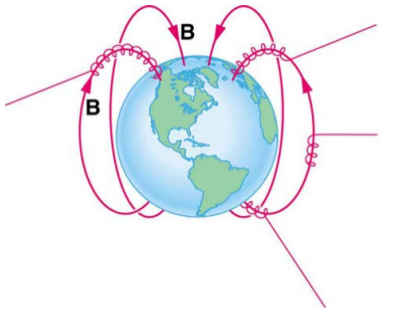
\includegraphics[width=0.45\textwidth]{figures/mag2.png}
\end{figure}
One un-explained piece: what does it mean for the electrons and protons to \textit{high-five} the neutral oxygen and nitrogen atoms?
\end{frame}

\section{Other forces}

\begin{frame}{Other forces}
The Lorentz force, when applied to a section of current-carrying wire, becomes
\begin{equation}
d\vec{F} = I \vec{dl} \times \vec{B}
\end{equation}
\begin{figure}
\centering
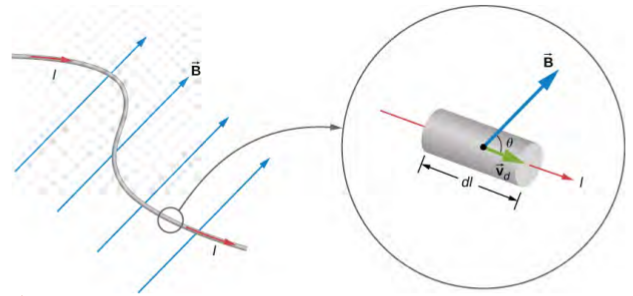
\includegraphics[width=0.55\textwidth]{figures/current.png}
\caption{\label{fig:current} The magnetic force on a section of current.}
\end{figure}
If the field is uniform:
\begin{equation}
\vec{F} = I \vec{L} \times \vec{B}
\end{equation}
\end{frame}

\begin{frame}{Other forces}
\small
\textbf{Group board exercise}: A wire of length 10 cm and mass 1 g is suspended in a horizontal plane by a pair of flexible leads.  The wire is then subjected to a constant magnetic field of magnitude 0.1 T, which is directed into the board.  What are the magnitude and direction of the current in the wire needed to remove the tension in the supporting leads?
\begin{figure}
\centering
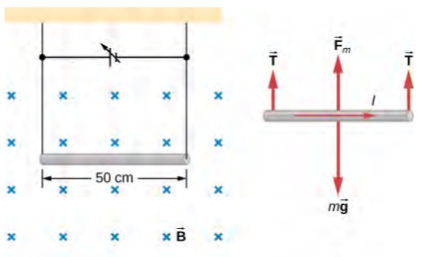
\includegraphics[width=0.5\textwidth]{figures/leads.png}
\caption{\label{fig:leads} Current suspended by Lorentz force...?}
\end{figure}
\end{frame}

\begin{frame}{Other forces}
Suppose a power supply provides the current in the previous example.  What if the voltage is raised, and the resistance stays constant, so that the current is doubled.  What will happen?
\begin{itemize}
\item A: The wire will rise.
\item B: The wire will fall.
\item C: The magentic field will decrease.
\item D: Nothing.
\end{itemize}
\end{frame}

\begin{frame}{Other forces}
If the wire is raised, what is doing the work to raise it?
\begin{itemize}
\item A: The wire will rise.
\item B: The wire will fall.
\item C: The magentic field will decrease.
\item D: Nothing.
\end{itemize}
\end{frame}

\begin{frame}{Other forces}
\small
\textbf{Group board exercise}: Suppose the current is raised from 1 amp to 2 amps for 0.1 seconds.  By how much will the wire be raised?  What is doing the work to raise this object?
\begin{figure}
\centering
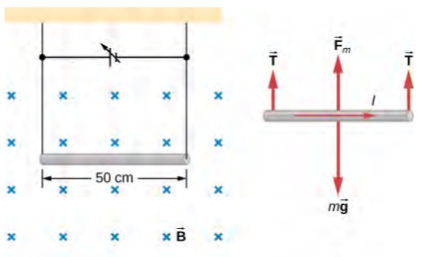
\includegraphics[width=0.5\textwidth]{figures/leads.png}
\caption{\label{fig:leads} Current suspended by Lorentz force...?}
\end{figure}
\end{frame}

\begin{frame}{Other forces}
\begin{figure}
\centering
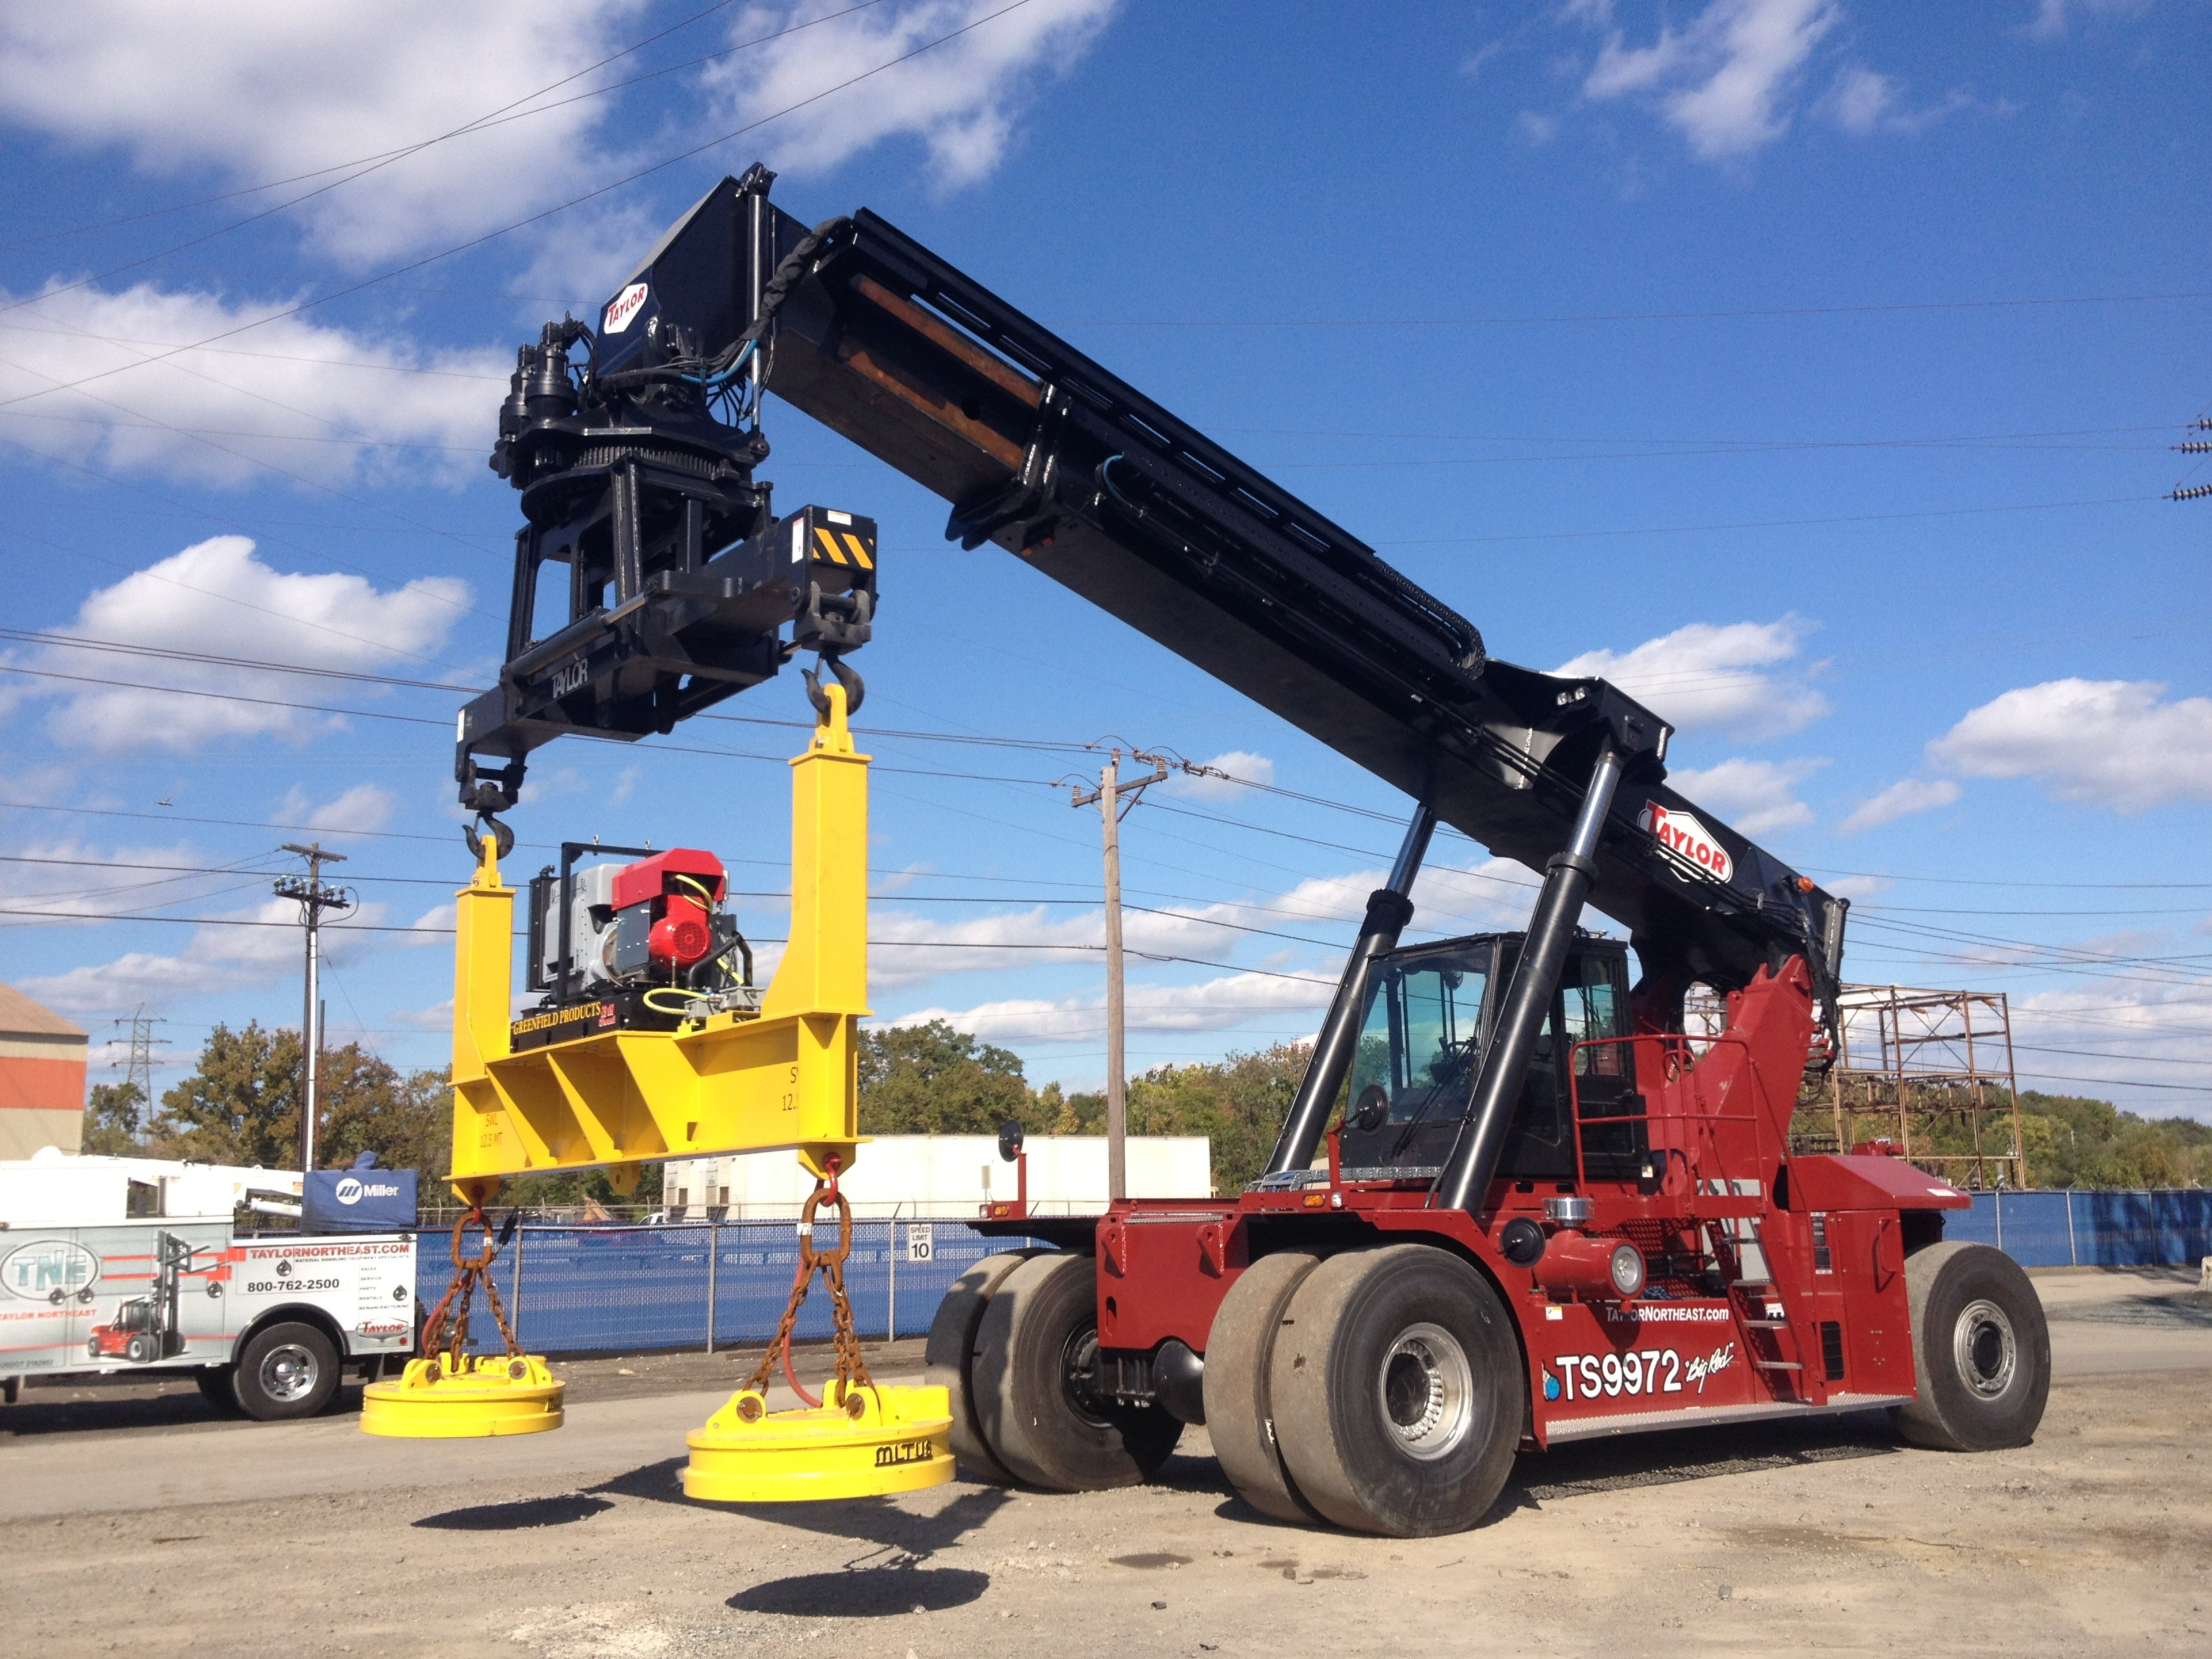
\includegraphics[width=0.5\textwidth]{figures/crane.jpg}
\caption{\label{fig:crane} An electromagnetic crane.}
\end{figure}
\end{frame}

\begin{frame}{Other forces}
\textbf{Observe on board.} The force is $F = dl I B \sin\theta$, but $dl = Rd\theta$.
\begin{figure}
\centering
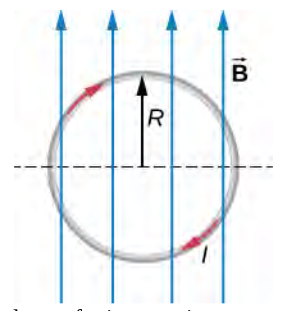
\includegraphics[width=0.4\textwidth,trim=0cm 0.1cm 0cm 0cm,clip=true]{figures/loop.png}
\caption{\label{fig:loop} Lorentz force on a loop of wire.}
\end{figure}
\end{frame}

\section{Conclusion}

\begin{frame}{Unit 5 Summary}
\textbf{Reading: Chapter 11}
\begin{enumerate}
\item Magnetism and magnetic fields
\item \alert{Motion of a charged particle in a magnetic field}
\item Other forces
\item Current loops
\end{enumerate}
\end{frame}

\section{Answers}

\begin{frame}{Answers}
\tiny
\begin{columns}[T]
\begin{column}{0.5\textwidth}
\begin{itemize}
\item Both A and B
\item 1 ms
\item 3.3 $\mu$ C
\item B and C
\item The particles have opposite charge, and about the same mass.
\item The wire will rise.
\end{itemize}
\end{column}
\begin{column}{0.5\textwidth}
\begin{itemize}
\item 
\end{itemize}
\end{column}
\end{columns}
\end{frame}

\end{document}
